\documentclass[12pt]{article}
\usepackage[a4paper, left=5mm, right=5mm, top=5mm, bottom=5mm]{geometry}
%\usepackage[a4paper, top=15mm, right=10mm, bottom=10mm, left=10mm]{geometry}
\usepackage[russian]{babel}
\usepackage{fontspec}
\usepackage{graphicx}
\usepackage[unicode]{hyperref}
\usepackage{enumitem}
\usepackage{wrapfig}
\usepackage{tabularx}
\usepackage{amssymb}
\usepackage{gensymb}
\usepackage{amsmath}
\usepackage{blindtext}
\usepackage{float}
\usepackage{multicol}
\usepackage{latexsym}
%\usepackage[font={bf}, name={Рис. }, justification=justified]{caption}
\usepackage{caption}
\usepackage{subcaption}
\usepackage{listings}
\usepackage{xcolor}
\usepackage{breqn}

\setmainfont{Times New Roman}
\righthyphenmin=2 % правильные переносы
\graphicspath{{images/}} % путь к картинкам

\newenvironment{enums}{\begin{enumerate}[leftmargin=0em,itemindent=3em, label=\textbf{\arabic*}]}{\end{enumerate}} % нужные перечисления

\definecolor{codegreen}{rgb}{0,0.6,0}
\definecolor{codegray}{rgb}{0.5,0.5,0.5}
\definecolor{codepurple}{rgb}{0.58,0,0.82}
\definecolor{backcolour}{rgb}{0.95,0.95,0.92}

% Стиль кода для 5 задания
\lstdefinestyle{mystyle}{
	backgroundcolor=\color{backcolour},   
	commentstyle=\color{codegreen},
	keywordstyle=\color{magenta},
	numberstyle=\tiny\color{codegray},
	stringstyle=\color{codepurple},
	basicstyle=\ttfamily\footnotesize,
	breakatwhitespace=false,         
	breaklines=true,                 
	captionpos=b,                    
	keepspaces=true,                 
	numbers=none,                    
	numbersep=5pt,                  
	showspaces=false,                
	showstringspaces=false,
	showtabs=false,                  
	tabsize=2
}
\lstset{style=mystyle}

\title{РГР МАТАН}
\author{Сиразетдинов, Шпинева, Лучинкин}


\begin{document}
	\thispagestyle{empty} % нет номеров страниц
\begin{center}
	Федеральное государственное автономное образовательное учреждение\\ 
	высшего образования\\
	«Национальный исследовательский университет ИТМО»\\
	\textit{Факультет Программной Инженерии и Компьютерной Техники}\\
\end{center}
\vspace{2cm}
\begin{center}
	\large
	Рассчетно-графическая работа\\
	по дисциплине математический анализ\\
	\textbf{Интеграл функции одной переменной}\\
	Модуль 2\\
	Вариант № 6
\end{center}
\vspace{7cm}
\begin{flushright}
	Выполнили:\\
	Сиразетдинов А. Н. P3116\\
	Шпинёва У. С. P3116\\
	Лучинкин К.\\
	Преподаватель: \\
	Возианова А. В.\\
\end{flushright}
\vspace{6cm}
\begin{center}
	г. Санкт-Петербург\\
	Университет ИТМО\\
	2023г.
\end{center}
	\newpage
	\tableofcontents
	\newpage
	\section{Задание 1. Интегральная сумма}
\subsection{Интегральная сумма}
\subsection*{Задание}
Исследуйте интегральную сумму функции $ \frac{1}{1 + x^2} $,заданной на отрезке $ \left[-1;\sqrt{3}\right]$
\subsection*{Интегральная сумма функции на заданном отрезке в виде ступенчатой фигуры}
\begin{center}
	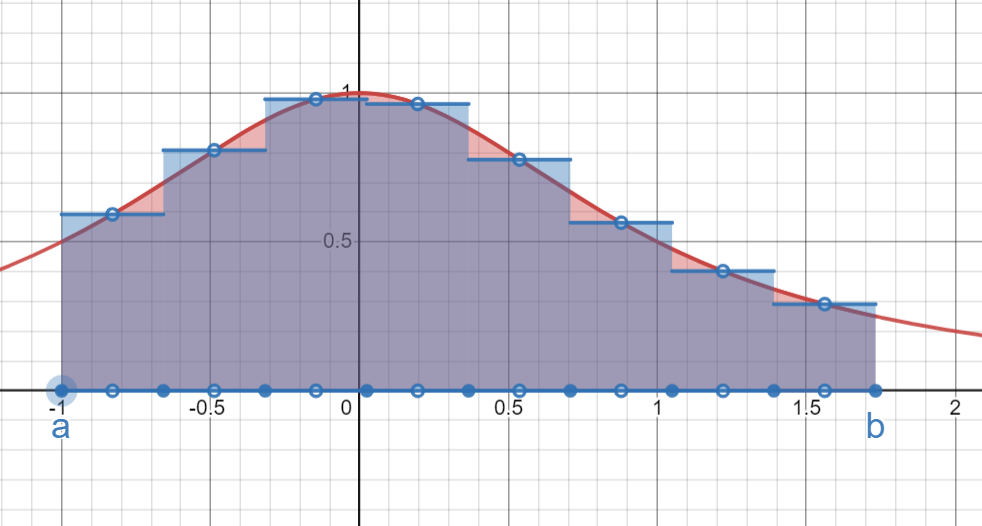
\includegraphics[width=0.4\linewidth]{task1/img1}\\
	\url{https://www.desmos.com/calculator/w21pp71fpr}
\end{center}
\subsection*{Исследование ступенчатой фигуры}
Рассмотрим разбиение на 3, 8 и 50 ступеней:
\begin{figure}[H]
	\centering
	\begin{subfigure}{0.3\textwidth}
		\centering
		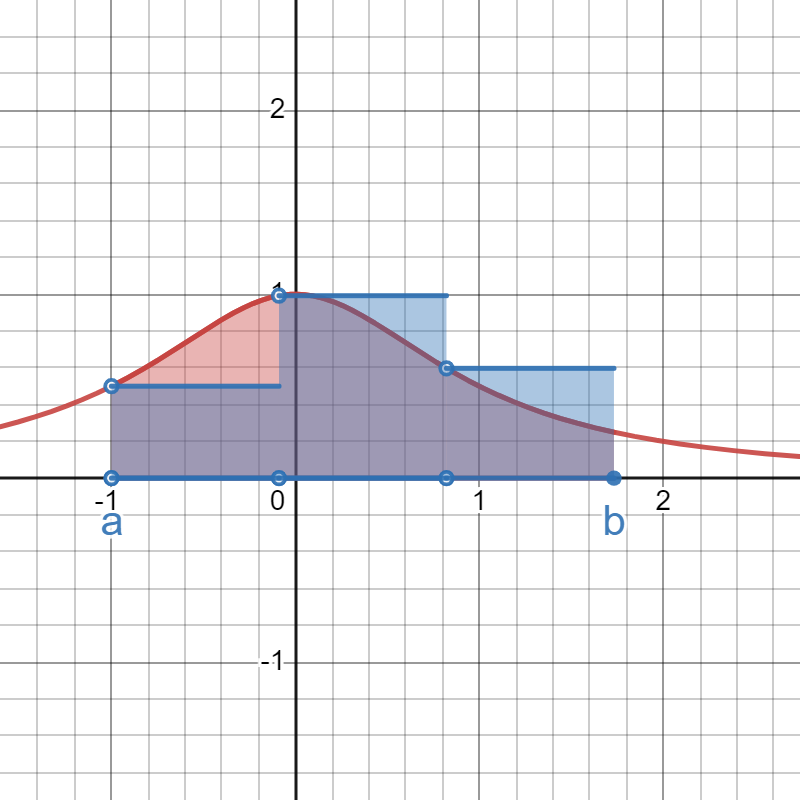
\includegraphics[width=.8\linewidth]{task1/n3/left}\quad
		\caption*{Крайнее левое положение точек}
	\end{subfigure}
	\begin{subfigure}{0.3\textwidth}
		\centering
		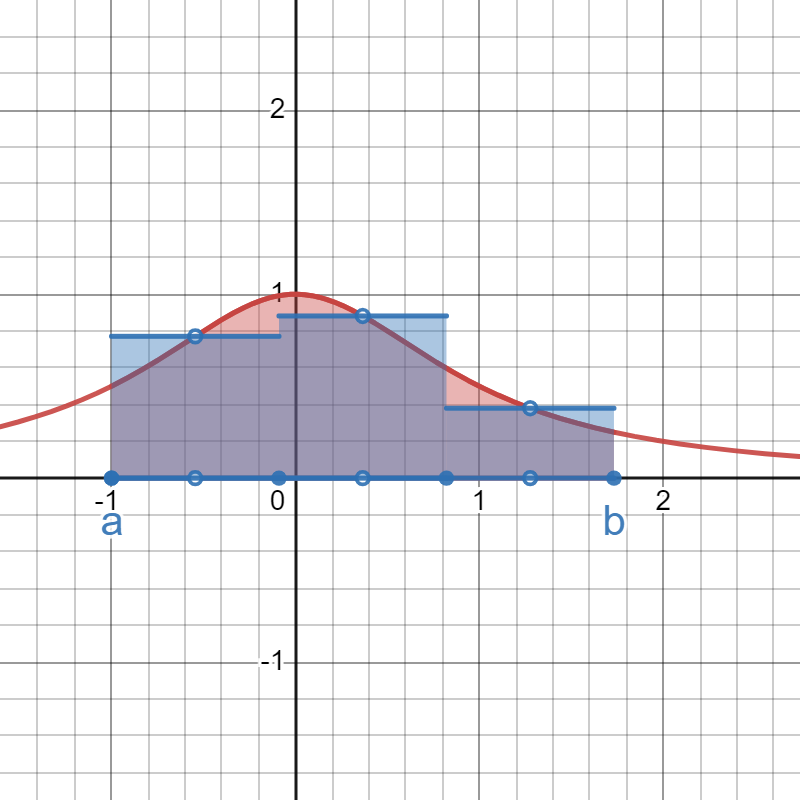
\includegraphics[width=.8\linewidth]{task1/n3/middle}\quad
		\caption*{Промежуточное положение точек}
	\end{subfigure}
	\begin{subfigure}{0.3\textwidth}
		\centering
		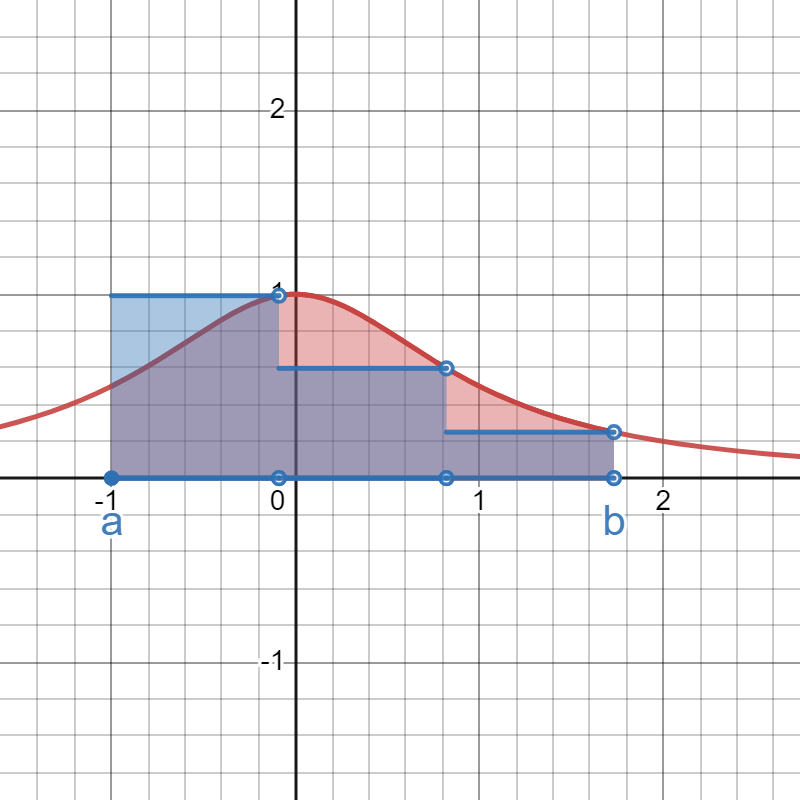
\includegraphics[width=.8\linewidth]{task1/n3/right}\quad
		\caption*{Крайнее правое положение точек}
	\end{subfigure}
	\caption{Разбиение на 3 ступени}
\end{figure}

\begin{figure}[H]
	\centering
	\begin{subfigure}{0.3\textwidth}
		\centering
		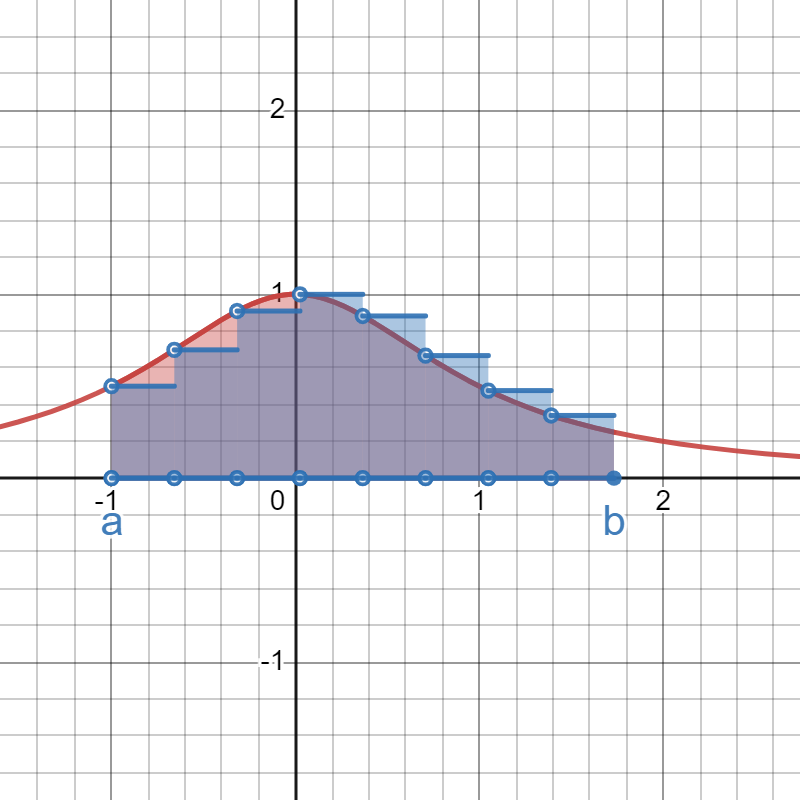
\includegraphics[width=.8\linewidth]{task1/n8/left}\quad
		\caption*{Крайнее левое положение точек}
	\end{subfigure}
	\begin{subfigure}{0.3\textwidth}
		\centering
		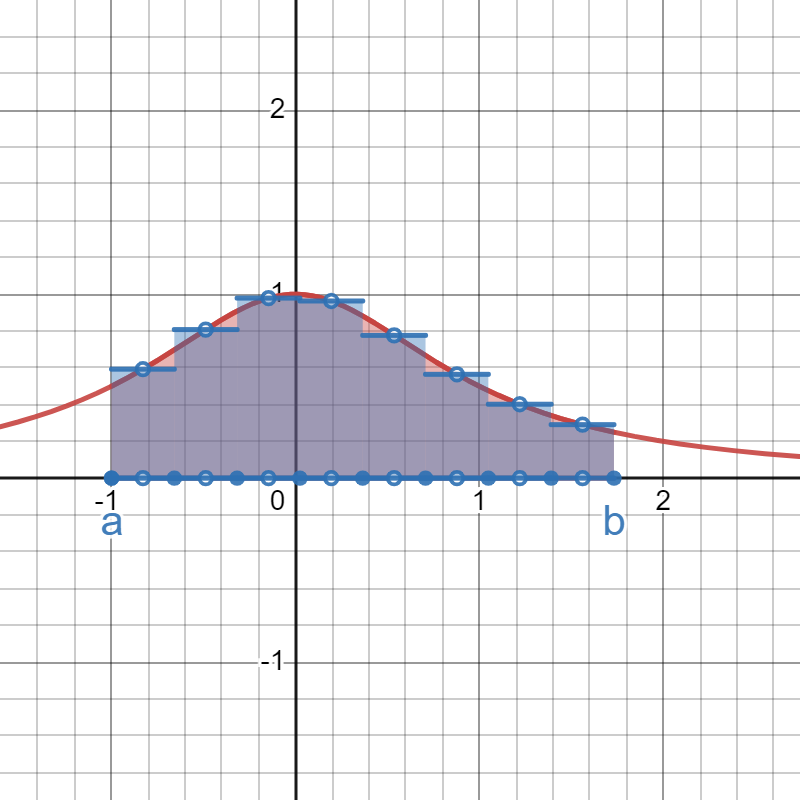
\includegraphics[width=.8\linewidth]{task1/n8/middle}\quad
		\caption*{Промежуточное положение точек}
	\end{subfigure}
	\begin{subfigure}{0.3\textwidth}
		\centering
		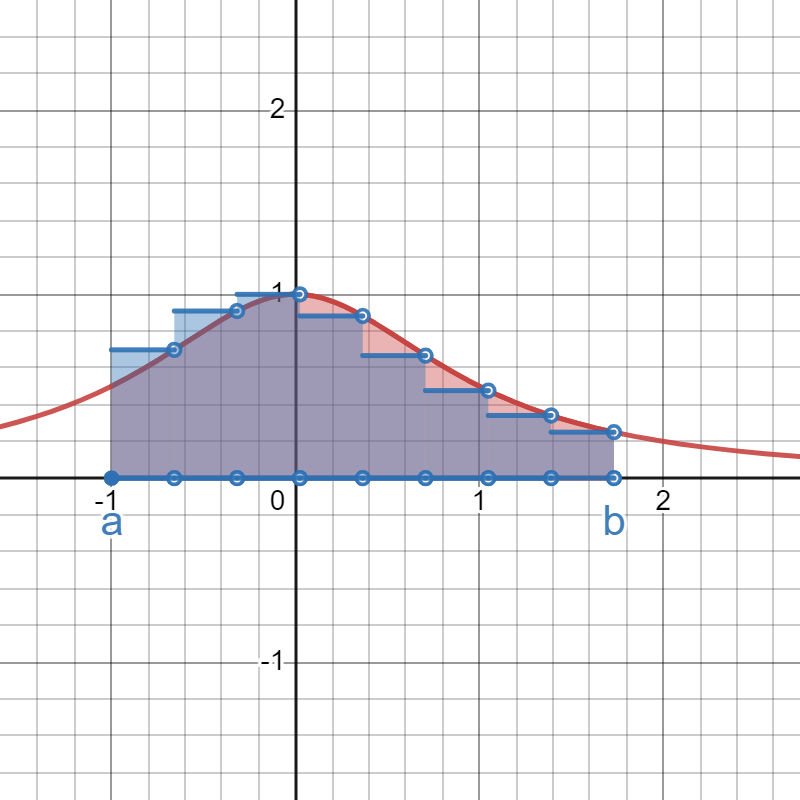
\includegraphics[width=.8\linewidth]{task1/n8/right}\quad
		\caption*{Крайнее правое положение точек}
	\end{subfigure}
	\caption{Разбиение на 8 ступеней}
\end{figure}

\begin{figure}[H]
	\centering
	\begin{subfigure}{0.3\textwidth}
		\centering
		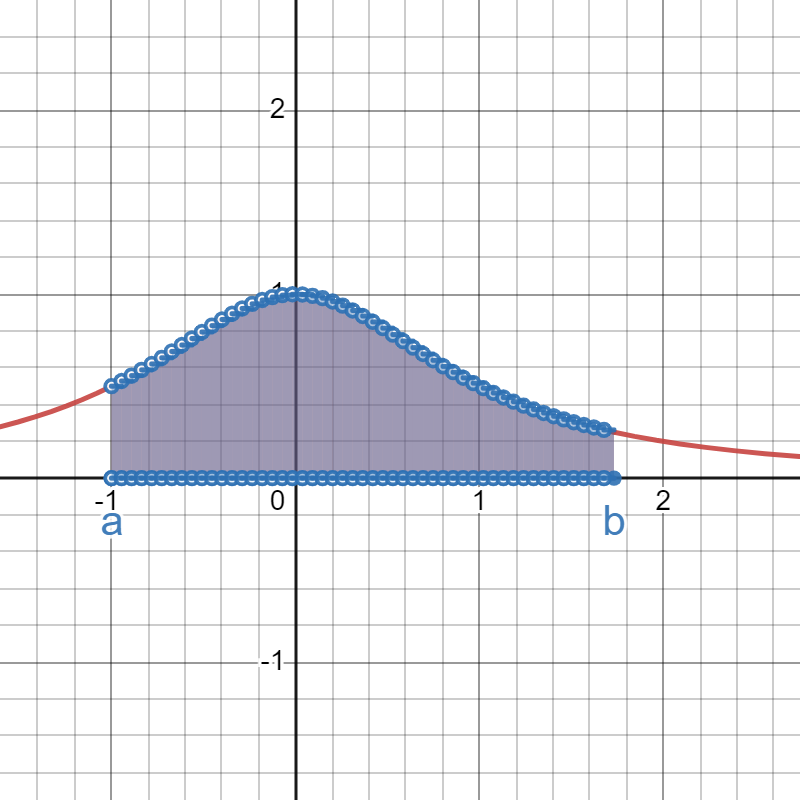
\includegraphics[width=.8\linewidth]{task1/n50/left}\quad
		\caption*{Крайнее левое положение точек}
	\end{subfigure}
	\begin{subfigure}{0.3\textwidth}
		\centering
		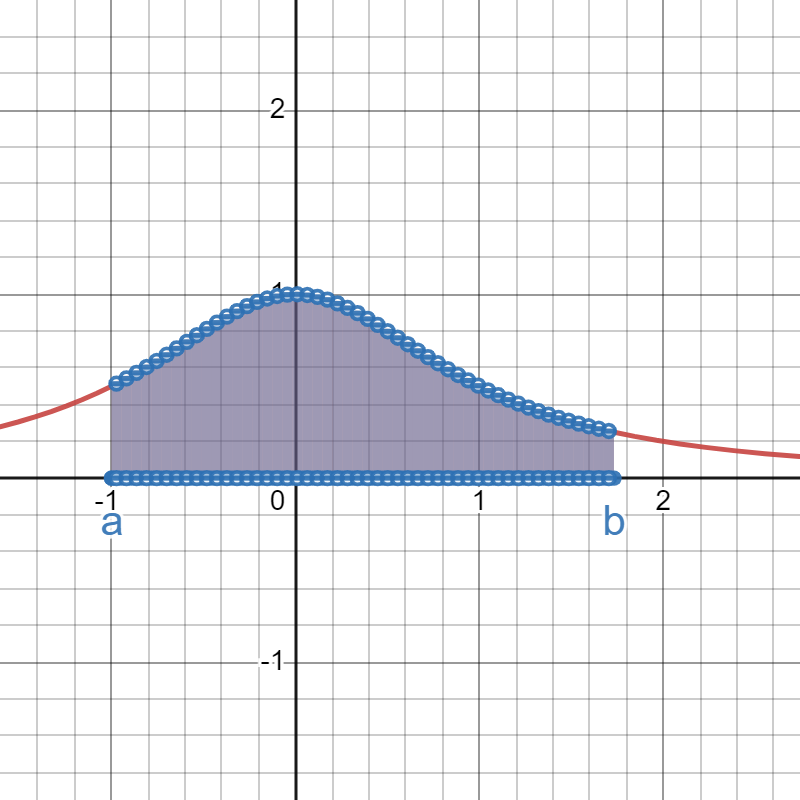
\includegraphics[width=.8\linewidth]{task1/n50/middle}\quad
		\caption*{Промежуточное положение точек}
	\end{subfigure}
	\begin{subfigure}{0.3\textwidth}
		\centering
		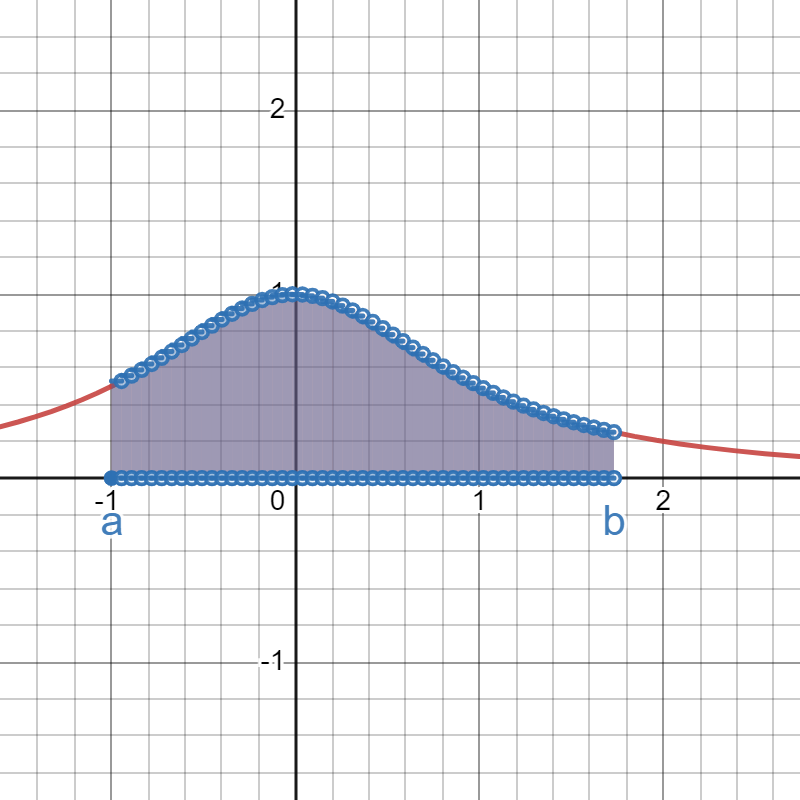
\includegraphics[width=.8\linewidth]{task1/n50/right}\quad
		\caption*{Крайнее правое положение точек}
	\end{subfigure}
	\caption{Разбиение на 50 ступеней}
\end{figure}
\subsection*{Заключение}
В процессе выполнения первой части первого задания были построены ступенчатые фигуры по графику. Ступенчатая фигура тем точнее, чем мельче разбиение и чем ближе выбранные точки к серединам разбиений
\subsection{Последовательность интегральных сумм}
\subsubsection*{Интегральная сумма}
\begin{figure}[H]
	\centering
	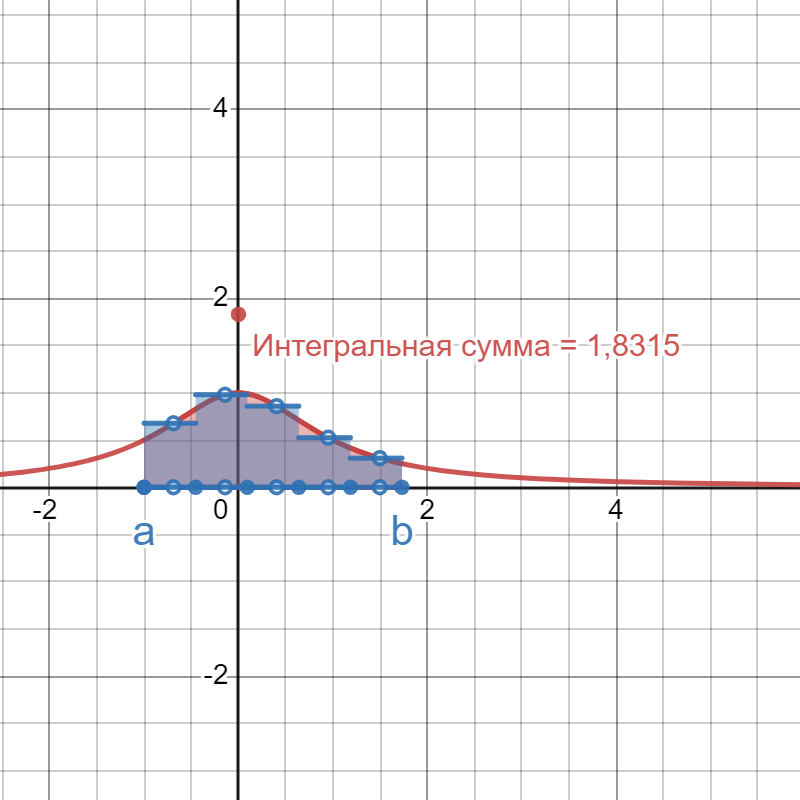
\includegraphics[width=0.4\linewidth]{task1/integrating_sums}\\
	\caption{Подсчет интегральной суммы}
\end{figure}
\subsubsection*{Исследование значения с ростом $ n $ при различных положениях точек}
\begin{figure}[H]
	\centering
	\begin{subfigure}{0.3\textwidth}
		\centering
		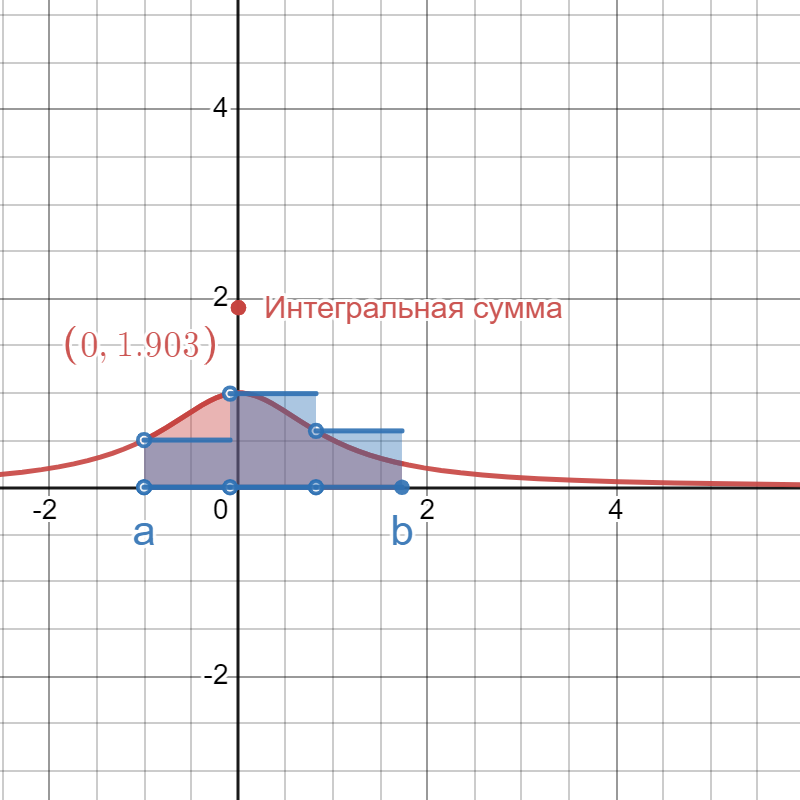
\includegraphics[width=.8\linewidth]{task1/sum_n3/left}\quad
		\caption*{Крайнее левое положение точек}
	\end{subfigure}
	\begin{subfigure}{0.3\textwidth}
		\centering
		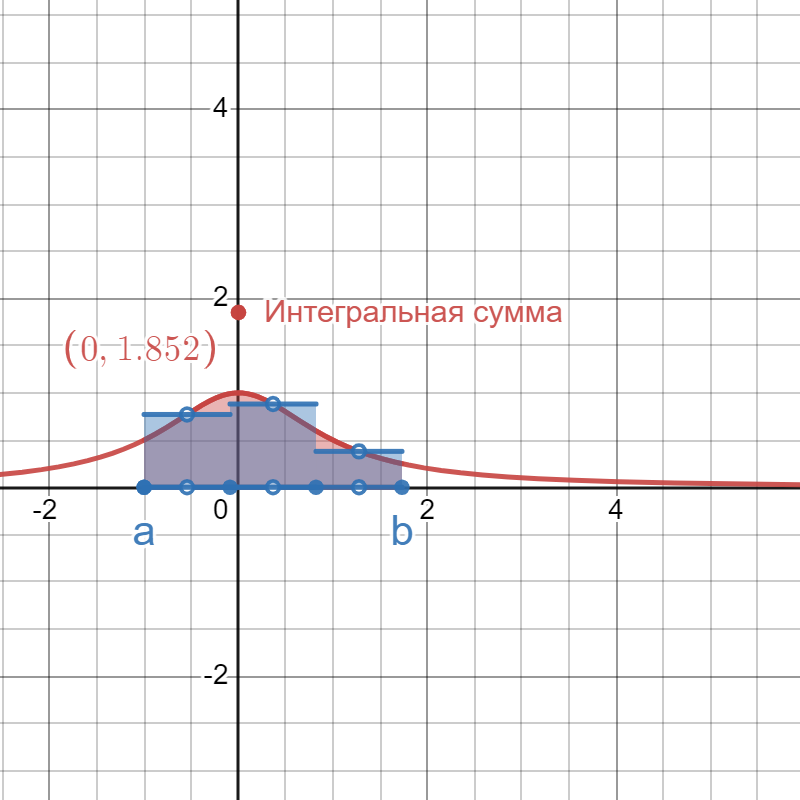
\includegraphics[width=.8\linewidth]{task1/sum_n3/middle}\quad
		\caption*{Промежуточное положение точек}
	\end{subfigure}
	\begin{subfigure}{0.3\textwidth}
		\centering
		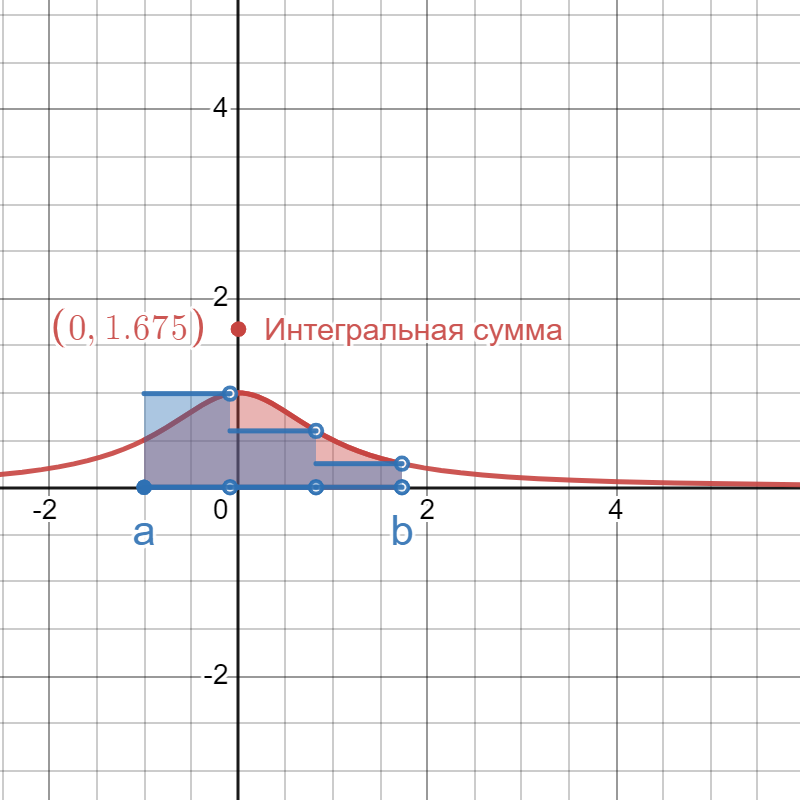
\includegraphics[width=.8\linewidth]{task1/sum_n3/right}\quad
		\caption*{Крайнее правое положение точек}
	\end{subfigure}
	\caption{Разбиение на 3 ступени}
\end{figure}

\begin{figure}[H]
	\centering
	\begin{subfigure}{0.3\textwidth}
		\centering
		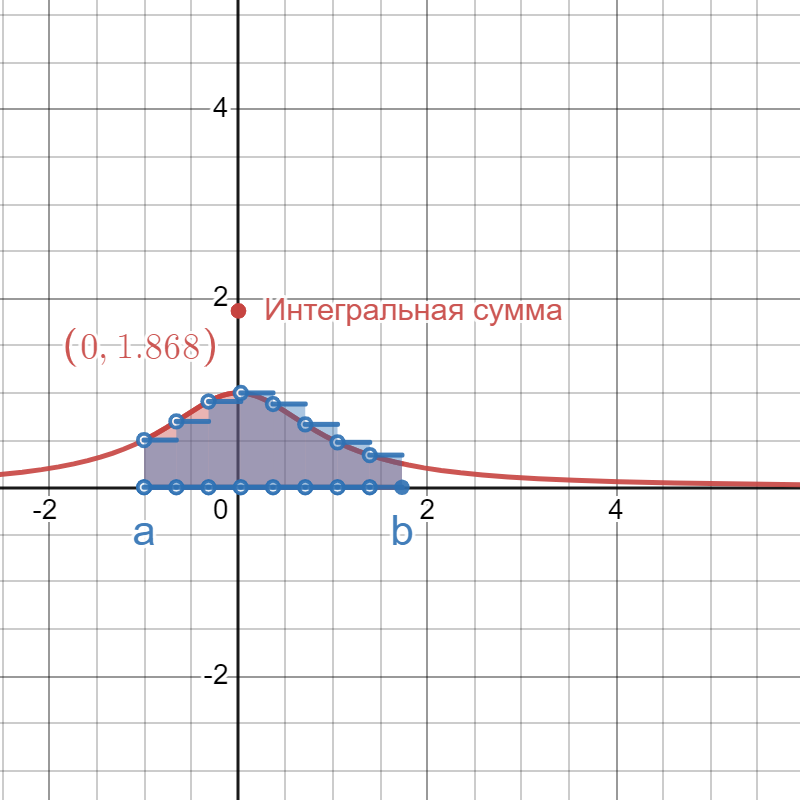
\includegraphics[width=.8\linewidth]{task1/sum_n8/left}\quad
		\caption*{Крайнее левое положение точек}
	\end{subfigure}
	\begin{subfigure}{0.3\textwidth}
		\centering
		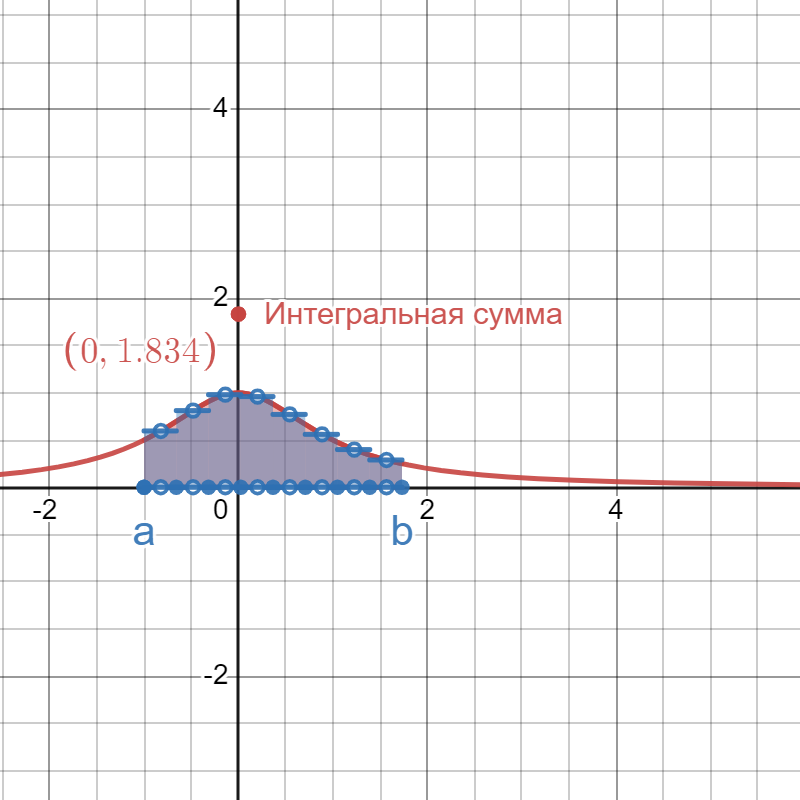
\includegraphics[width=.8\linewidth]{task1/sum_n8/middle}\quad
		\caption*{Промежуточное положение точек}
	\end{subfigure}
	\begin{subfigure}{0.3\textwidth}
		\centering
		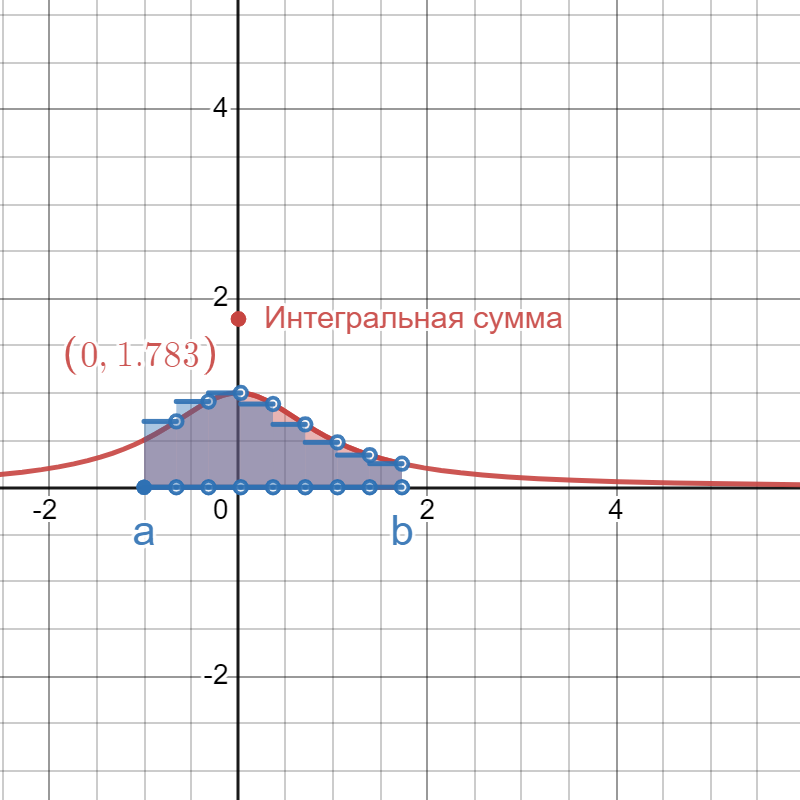
\includegraphics[width=.8\linewidth]{task1/sum_n8/right}\quad
		\caption*{Крайнее правое положение точек}
	\end{subfigure}
	\caption{Разбиение на 8 ступеней}
\end{figure}

\begin{figure}[H]
	\centering
	\begin{subfigure}{0.3\textwidth}
		\centering
		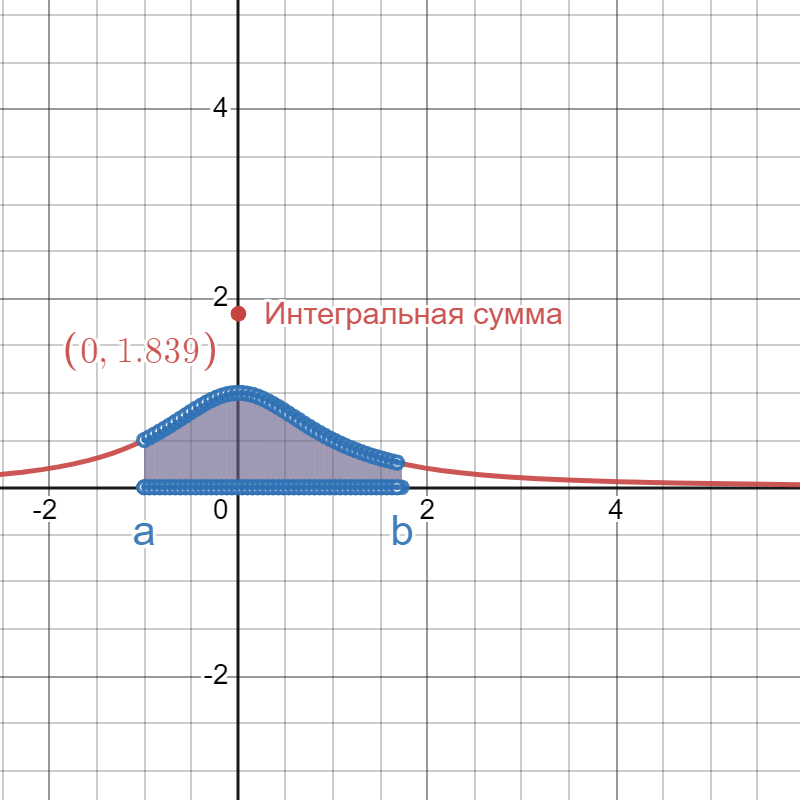
\includegraphics[width=.8\linewidth]{task1/sum_n50/left}\quad
		\caption*{Крайнее левое положение точек}
	\end{subfigure}
	\begin{subfigure}{0.3\textwidth}
		\centering
		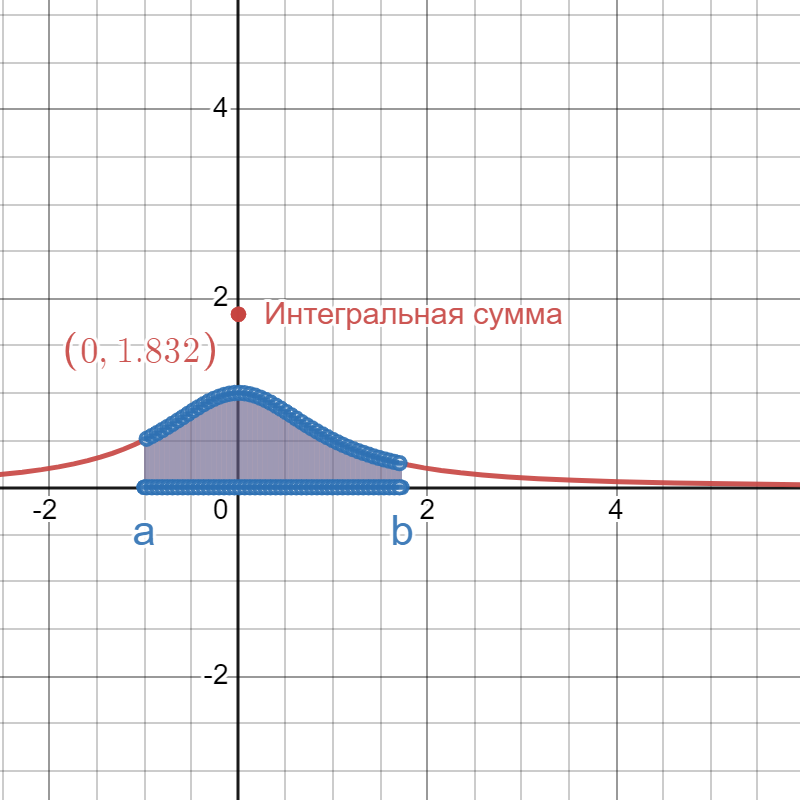
\includegraphics[width=.8\linewidth]{task1/sum_n50/middle}\quad
		\caption*{Промежуточное положение точек}
	\end{subfigure}
	\begin{subfigure}{0.3\textwidth}
		\centering
		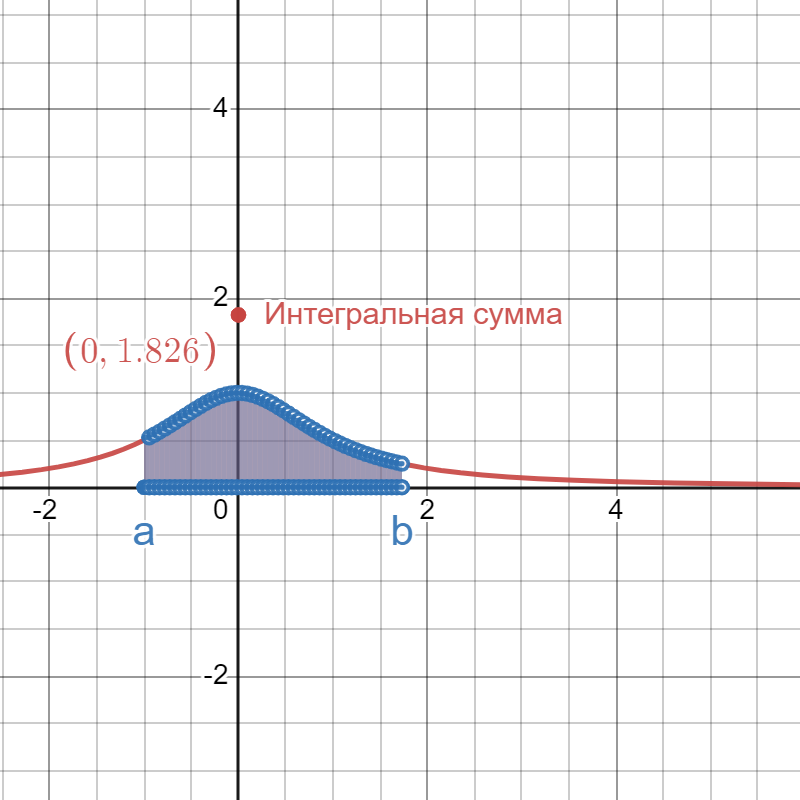
\includegraphics[width=.8\linewidth]{task1/sum_n50/right}\quad
		\caption*{Крайнее правое положение точек}
	\end{subfigure}
	\caption{Разбиение на 50 ступеней}
\end{figure}
\subsubsection*{Аналитическое вычисление интеграла}
\begin{equation*}
	\int_{-1}^{\sqrt{3}}\frac{dx}{1+x^2}=\arctg{x\bigg|_{-1}^{\sqrt{3}}}=\frac{\pi }{3}-\left(-\frac{\pi }{4}\right)=\frac{7\pi}{12}\approxeq1,8326
\end{equation*}
Интегральная сумма тем точнее, чем мельче разбиение и чем ближе выбранные точки к серединам разбиений
\subsubsection*{Последовательность интегральных сумм}
\begin{figure}[H]
	\centering
	\begin{subfigure}{0.3\textwidth}
		\centering
		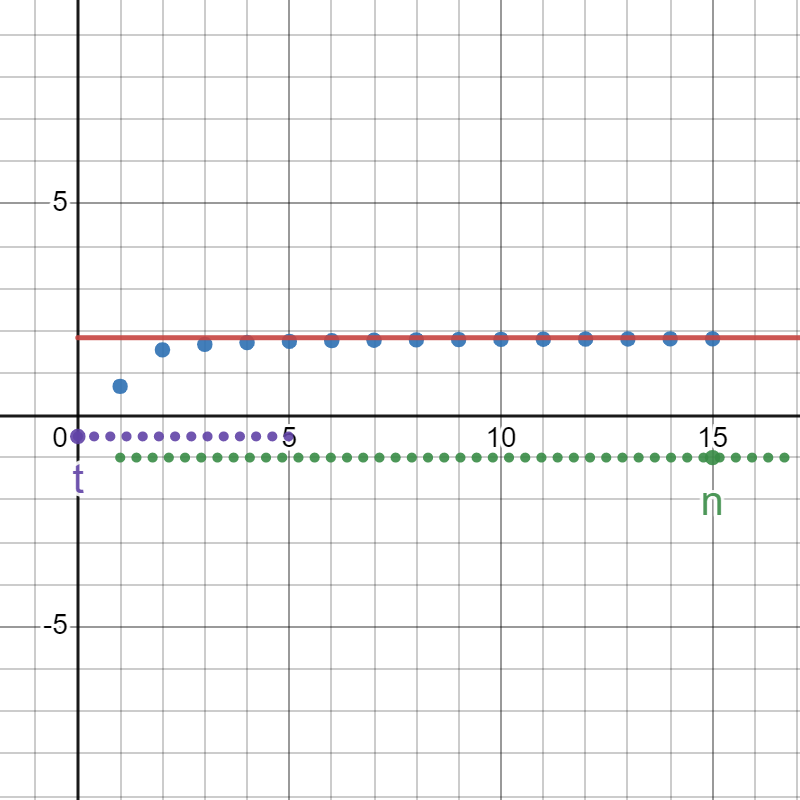
\includegraphics[width=.8\linewidth]{task1/sums/left}\quad
		\caption*{Крайнее левое положение точек}
	\end{subfigure}
	\begin{subfigure}{0.3\textwidth}
		\centering
		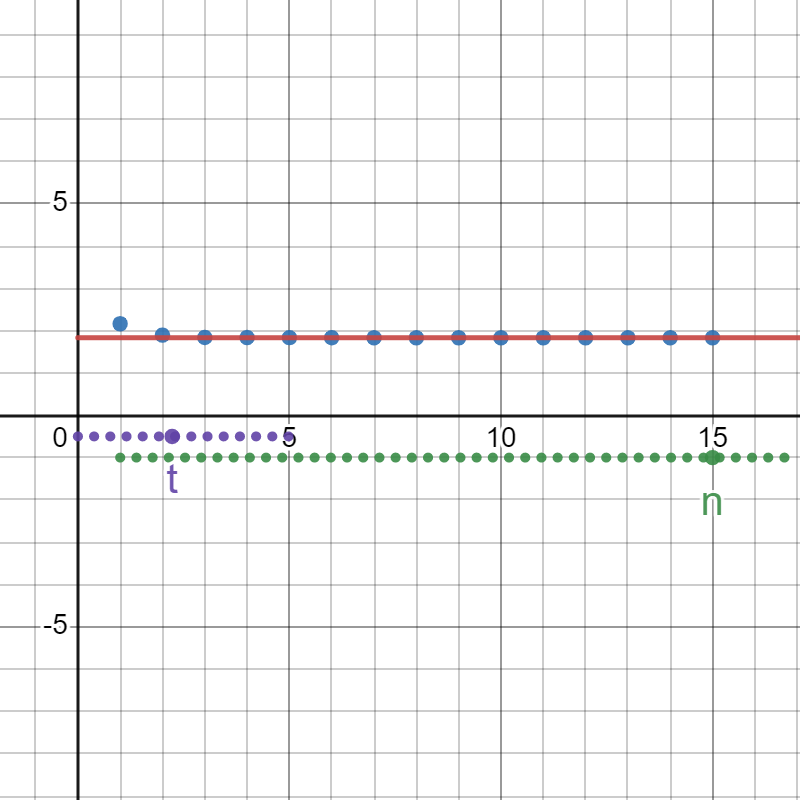
\includegraphics[width=.8\linewidth]{task1/sums/middle}\quad
		\caption*{Промежуточное положение точек}
	\end{subfigure}
	\begin{subfigure}{0.3\textwidth}
		\centering
		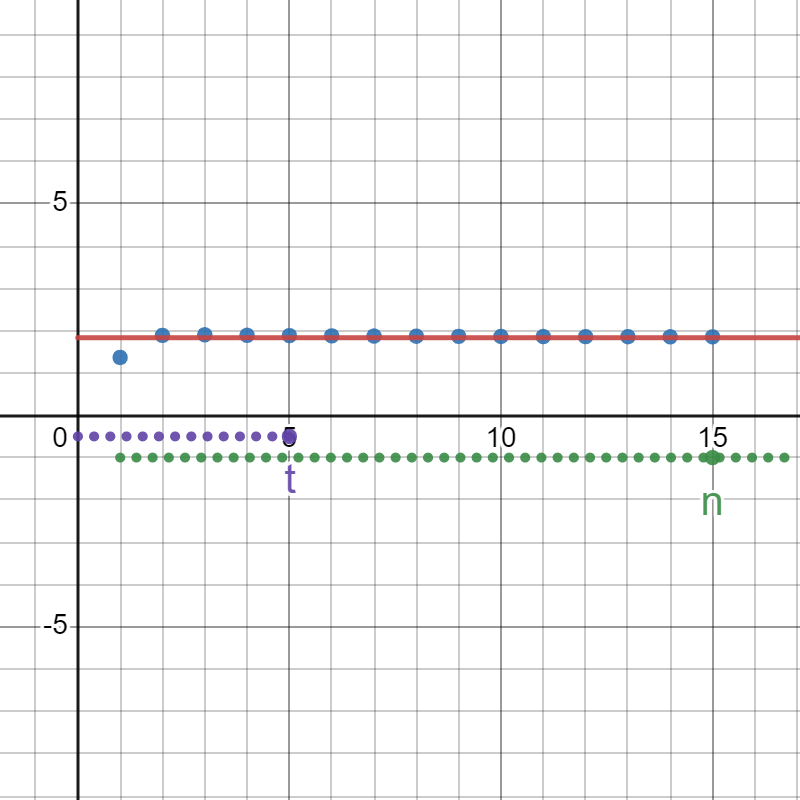
\includegraphics[width=.8\linewidth]{task1/sums/right}\quad
		\caption*{Крайнее правое положение точек}
	\end{subfigure}
	\caption{Зависимость от расположения точек}
	\url{https://www.desmos.com/calculator/zrwq9vbkt0}
\end{figure}
\subsubsection{Заключение}
В процессе выполнения части 2 задания 1 были сравнены значения интегральных сумм и аналитического исчисления. Можно сделать вывод, что вычисление определенного интеграла достаточно точное и его точность прямо пропорциональна количеству точек, которые мы выбираем и их близость к середине разбиений




	\newpage
	\section{Задание 2. Площадь фигуры}
\subsection*{Задание}
Найдите площадь фигуры, ограниченной кривой Лиссажу $x = 2sint$, $y = 2sin2t$
\subsection*{График кривой:}
\begin{center}
	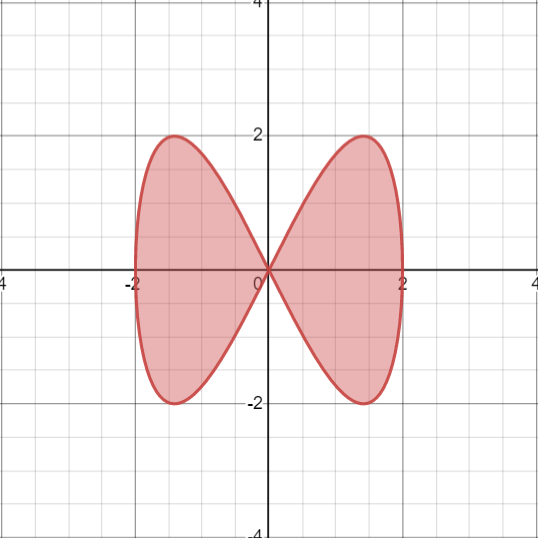
\includegraphics[width=0.4\linewidth]{task2_img1}\\
	\url{https://www.desmos.com/calculator/2y0dajpihq}
\end{center}
Кривая симметрична относительно обеих осей координат: если заменить $t$ на $(\pi - t)$, то переменная x не меняется, a $y$ изменяет только свой знак;
следовательно, кривая симметрична относительно оси $Ox$. При замене же $t$ на $(\pi + t)$ переменная $y$ не меняется, а $x$ меняет только свой знак. Это значит, что кривая симметрична относительно оси $Oy$.

В силу симметричности фигуры, для нахождения ее площади достаточно рассмотреть только четверть, значение на отрезке $[0, \frac{\pi}{2}]$ 
\begin{center}
	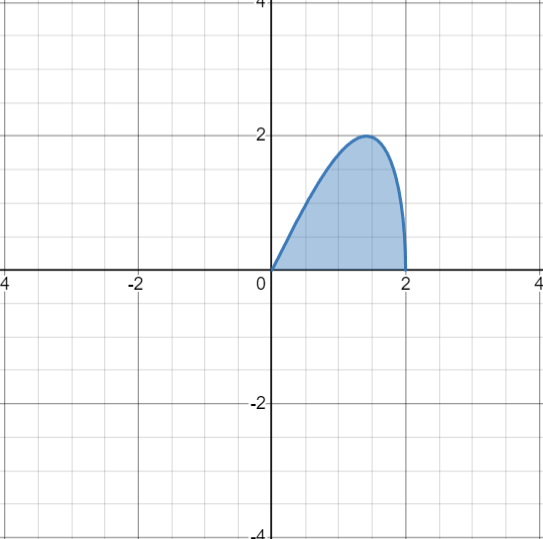
\includegraphics[width=0.4\linewidth]{task2_img2}\\
\end{center}

Тогда искомая
площадь будет равна полученному результату, умноженному на 4:\\
$S = 4 \int\limits_0^{\frac{\pi}{2}} y(x) x_t 'dt = 4 \int\limits_0^{\frac{\pi}{2}} 2 \cdot sin2t \cdot 2 \cdot cost dt = 16 \int\limits_0^{\frac{\pi}{2}} 2 \cdot sint \cdot cos^{2}t dt = -32 \int\limits_0^{\frac{\pi}{2}} cos^{2}t d(cost) = -32 \cdot {\frac{cos^{3}t}{3}} \bigg|_0^{\frac{\pi}{2}} = {\frac{32}{3}}$ 
	\newpage
	\section{Задание 3. Несобственный интеграл}
Исследуем сходимость \( \int_{1}^{\infty} \frac{dx}{(x^\alpha+ 1)arctg(x)} \)
Сравним ряд с \(\frac{1}{x^\alpha}\)
\begin{flalign*}
    &\lim_{x \to \infty} \frac{1}{(x^\alpha + 1)arctg(x)(\frac{1}{x^\alpha})} \le lim_{x \to \infty} \frac{1}{(x^\alpha + 1)\frac{\pi}{4}(\frac{1}{x^\alpha})},&\\
\end{flalign*}
Поскольку \(\arctg(x) \ge \frac{\pi}{4}\) на \([1,\infty)\)\\
\begin{flalign*}
    &\lim_{x \to \infty} \frac{1}{(x^\alpha + 1)\frac{\pi}{4}(\frac{1}{x^\alpha})} = \lim_{x \to \infty} \frac{x^\alpha}{\frac{\pi}{4}x^\alpha + \frac{\pi}{4}} = \frac{4}{\pi}
    &\\
\end{flalign*}
Тогда по предельному признаку сравнения \( \int_{1}^{\infty} \frac{dx}{(x^\alpha) + 1)\arctg(x)}\)  сходится или расходится одновременно с \(\int_{1}^{\infty} \frac{dx}{x^\alpha}\). Таким образом \(\int_{1}^{\infty} \frac{dx}{(x^\alpha) + 1)\arctg(x)} \) расходится при \(\alpha \leq 1\) и сходится при \(\alpha > 1\)
https://www.desmos.com/calculator/nmd2sx8waf
	\newpage
	\section{Задание 4. Приложения определенного интеграла}
Вычислить работу, необходимую для извлечения деревянной прямоугольной балки, плавающей в воде, если длина балки 5 м, ширина 40 см , высота 20 см, а ее удельный вес равен 0,8.\\
Удельный вес \(\gamma = \frac{P}{V}\), где P - вес балки, V - объём.\\
Поскольку балка плавает в воде вес балки равен весу воды, вытесняемой подводной частью балки.\\
т.е. \(0.8 \cdot (0.4 \cdot 5 \cdot 0.2) = 1 \cdot (0.4 \cdot 5 \cdot H)\), откуда \(H = 0.16\), , поскольку удельный вес воды - 1\\значит под водой находится 16см балки.\\
Чтобы достать балку из воды необходимо понять её на 16см = 0.16м.\\
F(h) - сила, которую надо приложить, чтобы поднять балку на высоту h.\\
\(F(h) = \gamma \cdot (0.4 \cdot 5 \cdot 0.2) - 1 \cdot (0.16-h) \cdot 0.4 \cdot 5\cdot \)
Таким образом, работа необходимую для извлечения балки \(A = \int_0^{0.1}(F(h))\)
\begin{flalign*}
&\int_0^{0.16} (0.32 - 2 (0.16 - h))dh = \int_0^{0.16} 2h dh = 0.0256 \text{Дж}&
\end{flalign*}
	\newpage
	\section{Задание 5. Приближенные вычисления определенного интеграла}
\subsection*{Задание}
Найти приближенное значение интеграла $ \int_0^{10}{e^{-x}	dx} = 0,999955 $ методами прямоугольников, трапеций, парабол , Боде при h=1. Сделать анализ полученных результатов.
\subsection*{Метод прямоугольников}
\begin{lstlisting}[language=Python]
def rectangle_method(f, a, b, n, t):
	h = (b - a) / n
	result = sum([f(a + (i - t) * h) for i in range(1, n + 1)]) * h
	return result
\end{lstlisting}
\subsection*{Метод трапеций}
\begin{lstlisting}[language=Python]
def trapezoid_method(f, a, b, n):
	h = (b - a) / n
	result = 0.5 * f(a) 
		+ sum([f(a + i*h) for i in range(1, n)]) 
		+ 0.5 * f(b)
	result *= h
	return result
\end{lstlisting}
\subsection*{Метод парабол}
\begin{lstlisting}[language=Python]
def parabola_method(f, a, b,n):
	h = (b - a) / n
	return (h / 3) * (sum([(f(a + h * (i - 1)) 
		+ 4 * f(a + h * i) 
		+ f(a + h * (i + 1))) for i in range(1, n, 2)]))
\end{lstlisting}
\subsection*{Метод Боде}
\begin{lstlisting}[language=Python]
def bode_method(f, a, b, h):
	splitting = [(a + h*i) for i in range(0, int((b - a) / h) + 1)]
	n = len(splitting)
	return (2 * h / 45 ) * (7 * (f(splitting[0]) + f(splitting[-1])) 
		+ 32 * (sum([f(splitting[i]) for i in range(1, n, 2)]))
		+ 12 * (sum([f(splitting[i]) for i in range(2, n - 1, 4)])) 
		+ 14 * (sum([f(splitting[i]) for i in range(4, n - 3, 4)])))
\end{lstlisting}
\url{https://colab.research.google.com/drive/1oaMYtnWpOiJltNrdXcKLQt34urXhq8pk?usp=sharing}
	\newpage
	\section{Задание 4. Приложение Рядов. Сиразетдинов Азат. Вариант 28}
\subsection{Задание 1}
Вычислить приближенно значение функции с точностью 0,0001 $ \cos48\degree $
\begin{eqnarray*} 
	&\text{Возьмем табличное разложение}\\
	&\cos x=  \sum_{k=0}^{\infty} (-1)^k \frac{x^{2k}}{(2k)!}\\
	&\cos48\degree = \cos(0,8378)\\
	&\text{1 член последовательности:}  \frac{0,8378^0}{1!} \approx 1\\
	&\text{2 член последовательности:}  (-1) * \frac{0,8378^2}{2!} \approx -0,35095\\
	&\text{3 член последовательности:}  \frac{0,8378^4}{4!} \approx 0,02052\\
	&\text{4 член последовательности:}  (-1) * \frac{0,8378^6}{6!} \approx -0,00048\\
	&\text{4 член последовательности:}  \frac{0,8378^8}{8!} \approx 0\\
	&\text{Дальнейшие члены не будут изменять точность}\\
	&\cos(0,8378) = 1 - 0,35095 + 0,02052 - 0,00048 \approx 0,66909 \approx 0,6691\\
\end{eqnarray*}
Проверка:
\begin{center}
	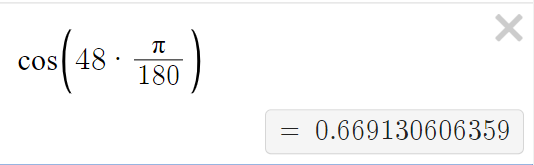
\includegraphics[width=.3\linewidth]{rgr2_task4_azat/cos_proof}\quad
\end{center}


	\newpage
	\linespread{1.3}
\section{Задание 4. Приложение Рядов. Шпинева Ульяна. Вариант 6}
\subsection{Задание 1}
Вычислить приближенно значение функции $ \frac{1}{\sqrt[3]{e^2}} $ с точностью 0,0001\\
\begin{flushright}
\begin{minipage}{15cm}
	\text{Возьмем табличное разложение}\\
	$e^x =  \sum_{k=0}^{\infty} \frac{x^n}{n!}$\\
	$e^{-\frac{2}{3}} =  \sum_{k=0}^{\infty} \frac{(-\frac{2}{3})^n}{n!}$\\
	\text{$n = 0:$}
	$$\frac{(-\frac{2}{3})^0}{0!} = 1$$\\
	\text{$n = 1:$}
	$$  \frac{(-\frac{2}{3})^1}{1!} \approx -0,66667 $$\\
	\text{$n = 2:$}
	$$\frac{(-\frac{2}{3})^2}{2!} \approx 0,22222$$\\
	\text{$n = 3:$}
	$$\frac{(-\frac{2}{3})^3}{3!} \approx -0,04938$$\\
	\text{$n = 4:$}
	$$\frac{(-\frac{2}{3})^4}{4!} \approx 0,00823$$\\
	\text{$n = 5:$}
	$$\frac{(-\frac{2}{3})^5}{5!} \approx -0,00109$$\\
	\text{$n = 6:$}
	$$\frac{(-\frac{2}{3})^6}{6!} \approx 0,00012$$\\
	\text{$n = 7:$}
	$$\frac{(-\frac{2}{3})^7}{7!} \approx -0,00001$$\\
\end{minipage}\\
\end{flushright}
	\text{Дальнейшие члены не будут изменять точность}\\
	 $ \frac{1}{\sqrt[3]{e^2}} \approx 1 - 0,66667 + 0,22222 - 0,04938 + 0,00823 - 0,00109 + 0,00012 - 0,00001 = 0,51342 $\\

Проверка:
\begin{center}
	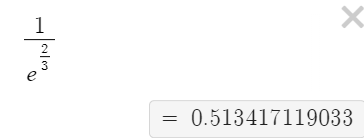
\includegraphics[width=.3\linewidth]{1_proof.png}\quad
\end{center}
\newpage
\subsection{Задание 2}
Разлагая подынтегральную функцию в степенной ряд вычислить приближенно интеграл с точностью 0,0001\\
\begin{equation*}
	\int_0^{\frac{1}{2}}ln(1 + x^4) dx
\end{equation*}
\begin{flalign*} 
	&\text{Возьмем табличное разложение}&&\\
	&\int_0^{\frac{1}{2}} ln(1 + x^4) dx = 
	\int_0^{\frac{1}{2}} \sum_{n=1}^\infty \frac{(-1)^{n-1} x^{4n}}{n} dx =
	\sum_{n=1}^\infty \int_0^{\frac{1}{2}} \frac{(-1)^{n-1} x^{4n}}{n} dx = 
	=\sum_{n=1}^\infty \frac{(-1)^{n-1}x^{4n+1}}{n(4n+1)} \bigg|_0^{\frac{1}{2}} =  &&\\
	&\sum_{n=1}^\infty \frac{(-1)^{n-1}}{n2^{4n+1}(4n+1)} &&\\
\end{flalign*}

Подсчитаем первые члены последовательности:
\begin{flalign*} 
	\text{$n = 1:$}& &&\\
	&\frac{1}{2^{5}\cdot 5} \approx 0,00625&&\\
	\text{$n = 2:$}& &&\\
	&\frac{-1}{2 \cdot 2^{9} \cdot 9} \approx -0,00011&&\\
	\text{$n = 3:$}& &&\\
	&\frac{1}{3 \cdot 2^{13} \cdot 13} \approx 0&&\\
	\text{Дальнейшие члены не будут изменять точность}& &&\\
	\int_0^{\frac{1}{2}}ln(1 + x^4) dx \approx 0,00625 &- 0,00011 = 0,00614
\end{flalign*}

Проверка:
\begin{center}
	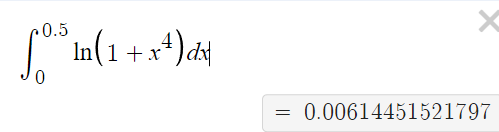
\includegraphics[width=.3\linewidth]{2_proof}\quad
\end{center}

\subsection{Задание 3}
Найти в виде степенного ряда решение дифференциального уравнения,
удовлетворяющего заданным начальным условиям. Ограничиться четырьмя
членами ряда.
\begin{flalign*}
	&y' = y^2 - 3x \\
	&y(1) = 2 \\
\end{flalign*}
\begin{flalign*}
	\text{Решение в виде ряда Тейлора: }& &&\\
	&y(x) = y(1) + y'(1)(x - 1) + \frac{y''(1)(x - 1)^2}{2!} + \frac{y'''(1)(x - 1)^3}{3!}&&\\
	1) \ &y' = y^2 - 3x &&\\
	&y'(1) = 2^2 - 3 = 1 &&\\
	2) \ &y'' = (y^2 - 3x)' = 2yy' - 3 &&\\
	&y''(1) = 2 \cdot 2 \cdot 1 - 3 = 1 &&\\
	3) \ &y''' = (2yy' - 3)' =  2y'y' + 2yy''&&\\
	&y'''(1) = 2 \cdot 1 \cdot 1 + 2 \cdot 2\cdot 1 = 6 &&\\
	\text{Подставим значения в ряд: }& &&\\
	&y(x) = y(1) + y'(1)(x - 1) + \frac{y''(1)(x - 1)^2}{2!} + \frac{y'''(1)(x - 1)^3}{3!} = &&\\
	&= 2 + (x - 1) + \frac{(x - 1)^2}{2} + (x - 1)^3 &&\\
\end{flalign*}

	\newpage
	\section{Лучинкин Константин индивидуальное задание.}
\subsection{Задание 1.}
\begin{flalign*}
& f(x) = e^x &
\end{flalign*}
Требуется посчитать \(f(-\frac{9}{10}) = \frac{1}{\sqrt[10]{e^9}}\)\\
Разложим \(f(x)\) в ряд Тейлора:
\begin{flalign*}
&f(x) = \sum_{n=0}^\infty \frac{x^n}{n!}&
\end{flalign*}
Рассмотрим частичные суммы рядя \(S_{(N,x)} = \sum_{n=0}^N \frac{x^n}{n!}\):\newline
\begin{flalign*}
& S_{(1, x)} = 1 + x;\quad S_{(1, -0.9)} = 0.1 &\\
& S_{(2, x)} = 1 + x + \frac{x^2}{2};\quad S_{(2, -0.9)} = 0.505 &\\
& S_{(3, x)} = 1 + x + \frac{x^2}{2} + \frac{x^3}{6};\quad S_{(3, -0.9)} = 0.3835 &\\
&...&\\
& S_{(7, x)} = \sum_{n=0}^7 \frac{x^7}{7!};\quad S_{(7, -0.9)} \approx 0.40655 &\\
& S_{(8, x)} = \sum_{n=0}^8 \frac{x^8}{8!};\quad S_{(8, -0.9)} \approx 0.40657 &
\end{flalign*}
Таким образом \(f(x) \approx 0.4065\) (с точностью до 0.0001)
\subsection{Задание 2}
\begin{flalign*}
    &\int_0^1 \frac{x^2dx}{\sqrt[4]{16 + x^4}}&\\
    &\text{Разложим }f(x) \text{ в ряд:}&\\
    &f(x) = \frac{x^2}{\sqrt[4]{16 + x^4}} = \frac{x^2}{2\sqrt[4]{\frac{x^4}{16} + 1}} = \frac{x^2}{2}\Big(\frac{x^4}{16}+1\Big)^{-\frac{1}{4}} = \frac{x^2}{2}\Big(1 + \sum_{n=0}^\infty \frac{\prod_{i=1}^{n-1}\Big(-\frac{1}{4}-i\Big)}{n!}\Big(\frac{x^4}{16}\Big)^n\Big)&\\
    &\int_0^1 \Big(\frac{x^2}{2}\Big)dx \approx 0.1666&\\
    &\int_0^1 \Big(\frac{x^2}{2} - \frac{x^6}{128}\Big)dx \approx 0.1655 &\\
    &\int_0^1 \Big(\frac{x^2}{2} - \frac{x^6}{128} + \frac{5x^{10}}{16384}\Big)dx \approx 0.1655 
\end{flalign*}
Таким образом \(\int_0^1 \frac{x^2dx}{\sqrt[4]{16 + x^4}} \approx 0.1655\) (с точностью до 0.0001)
\subsection{Задание 3}
Найти в виде степенного ряда решение дифференциального уравнения,
удовлетворяющего заданным начальным условиям. Ограничиться четырьмя
членами ряда.
\begin{flalign*}
    &y'' = e^{y-2}\ln y' + x &\\
    &y(3) = 2 &\\
    &y'(3) = 1&
\end{flalign*}
Запишем формулу Тейлора для \(x=3\):
\begin{flalign*}
    &f(x) = y(3) + y'(3)(x-3) + y''(3)(x-3)^2&\\
    &y''(3) = e^{y(3)-2}\ln y'(3) + 3 = 3&\\
    &f(x) = 2 + (x-3) + 3(x-3)^2 + r_n\quad \quad \quad \quad r_n \text{-остаточный член}&
\end{flalign*}
	\newpage
	\linespread{1.3}
\section{Задание 3. Ряд Тейлора}
\subsection{Задание}
Исследуйте ряд Тейлора функции  в точке. Изобразите графически несколько различных  частичных сумм ряда и график исходной функции. Проведите анализ полученных результатов.\\
\begin{equation*}
	f(x) = ln(\frac{x - 2}{7 - 2x}), \quad x_0 = 3
\end{equation*}
\begin{flalign*} 
	&\text{Найдем первые 5 производных и их значения в точке x_0}&&\\
	&f(3) = ln(1) = 0&&\\
	1) \ &f'(x) = \frac{3}{(x - 2)(7 - 2x)} &&\\
	&f'(3) = 3 &&\\
	2) \ &f''(x) = \frac{12x - 33}{(-2x^2 + 11x - 14)^2} &&\\
	&f''(3) = 3 &&\\
	3) \ &f'''(x) = \frac{72x^2 - 396x + 558}{(-2x^2 + 11x - 14)^3}&&\\
	&f'''(3) = 18 &&\\
	4) \ &f^{IV}(x) = \frac{576x^3 - 4752x^2 + 13392x - 12870}{(-2x^2 + 11x - 14)^4}&&\\
	&f^{IV}(3) = 90 &&\\
	5) \ &f^{V}(x) = \frac{5760x^4 - 63360x^3 + 267840x^2 - 514800x + 378792}{(-2x^2 + 11x - 14)^5}&&\\
	&f^{V}(3) = 792 &&\\
	\text{Подставим значения в ряд: }& &&\\
	&f(x) = y(3) + y'(3)(x - 3) + \frac{y''(3)(x - 3)^2}{2!} + \frac{y'''(3)(x - 3)^3}{3!} + \frac{y^{IV}(3)(x - 3)^4}{4!} + &&\\
	& + \frac{y^{V}(3)(x - 3)^5}{5!} + \dots = &&\\
	&= 0 + 3 \cdot (x - 3) + 3 \cdot \frac{(x - 3)^2}{2!} + 18 \cdot \frac{(x - 3)^3}{3!} + 90 \cdot \frac{(x - 3)^4}{4!}  + 792 \cdot \frac{(x - 3)^5}{5!}  + \dots = &&\\
	&= 0 + 3 \cdot (x - 3) + \frac{1 \cdot 3}{2} \cdot (x - 3)^2 + \frac{3 \cdot 3}{3} \cdot (x - 3)^3 + \frac{5 \cdot 3}{4} \cdot (x - 3)^4 &&\\
	&+ \frac{11 \cdot 3}{5} \cdot (x - 3)^5  + \dots = &&\\
	&= \sum_{n=1}^\infty \frac{2^n + (-1)^{n + 1}}{n}(x - 3)^n&& \\
\end{flalign*}
\begin{flalign*}
	&\text{Найдем область сходимости:}&&\\
	& R = \lim_{n \to \infty} \bigg|\frac{c_n}{c_{n + 1}}\bigg| = \lim_{n \to \infty} \bigg|\frac{(2^n + (-1)^{n + 1})(n + 1)}{n(2^{n + 1} + (-1)^{n + 2})}\bigg| = \frac{1}{2} &&\\
	&\text{Рассмотрим граничные точки:}&&\\
	&\frac{1}{2^n} \cdot \frac{2^n + (-1)^{n + 1}}{n} \geq \frac{1}{2^n} \cdot \frac{2^n - 1}{n}&&\\
	&\text{Сравним ряд с гармоническим:}&&\\
	& \lim_{n \to \infty} \frac{\frac{2^n - 1}{2^n \cdot n}}{\frac{1}{n}} = 1  => \text{ряд расходится}&&\\
	&\frac{1}{(-2)^n} \cdot \frac{2^n + (-1)^{n + 1}}{n}&&\\
	&\text{Рассмотрим первые 3 члена ряда:}&&\\
	&-\frac{3}{2}, \frac{3}{8}, -\frac{3}{8}&&\\
	&\text{Модуль каждого последующего члена ряда не меньше предыдущего, а значит ряд расходится по признаку}&&\\
	&\text{Лейбница}&&\\
	&\text{Таким образом область сходимости исходного ряда: } (2,5; 3,5)&&\\
\end{flalign*}
\begin{center}
	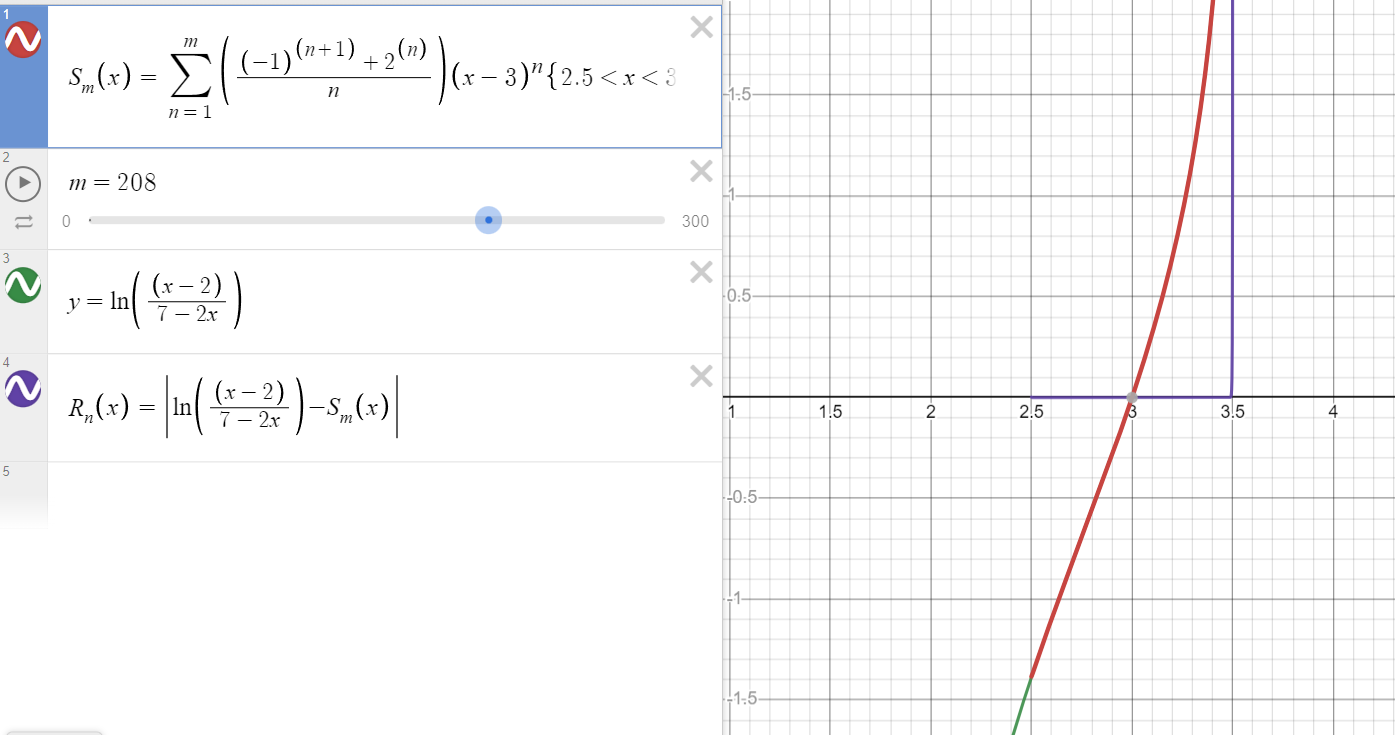
\includegraphics[width=0.9\linewidth]{task2_1_img1}\\
	\url{https://www.desmos.com/calculator/8d2svsbywe?lang=ru}
\end{center}

	\newpage
	\section{Задание 3.}
Разложим функцию в ряд:
\begin{flalign*}
&f(x) = ln\Bigr(\frac{x-2}{7 - 2x}\Bigl) = ln((x-3)+1) - ln((6-2x)+1) = &\\
&\sum_{n=1}^{\infty} (-1)^{(n-1)} \frac{(x-3)^n}{n!} - \sum_{n=1}^{\infty} (-1)^{(n-1)} \frac{(6-2x)^n}{n!} = \sum_{n=1}^{\infty} (-1)^{(n-1)} \frac{(x-3)^n}{n!} + \sum_{n=1}^{\infty}\frac{2^n(3-x)^n}{n!} = &\\
& = \sum_{n=1}^{\infty} ((-1)^{(n-1)} + 2^n) \frac{(x-3)^n}{n!}^{(*)}
\end{flalign*}
Найдём область сходимости ряда. \( \sum_{n=1}^{\infty}\) сходится на \((-1,1]\). Тогда для того, чтобы найти область сходимости \((*)\) решим систему уравнений:\newline
\[
\begin{cases}
-1 < x-3 \le 1\\
-1 < 6 - 2x \le 1
\end{cases}
\iff
\begin{cases}
2 < x \le 4\\
3.5 > x \ge 2.5
\end{cases}
\iff
2.5 \le x < 3.5
\]\newline
Гафик функции и бесконечного ряда:
https://www.desmos.com/calculator/j07rbqxznf

\end{document}